In order to extract the shape of the $m_{4\ell}$ distribution for the reducible background used in the final analysis, 
shapes for each category and each final state are studied in the mass range [70, 300] GeV in both the SS and OS methods using 2016 dataset. 
Then the standard [105, 140] GeV window is used in the final analysis.

The study is focused on the SS method because of the better statistics available. 
A fit to Landau function is performed to provide the $m_{4\ell}$ shape in each category separately for the $4e$, $4\mu$, $2\mu2e$ and $2e2\mu$ final state, 
as shown in Figure~\ref{fig:shapes}. 
Since not all the categories are populated enough, the minimum number of events needed to extract the shape for a single category has been evaluated; 
therefore, in the very low populated categories (less than fifty events selected in the mass window) 
shapes obtained from the inclusive distributions in each final state are used.
%
%\begin{figure}[h]
%\begin{center}
%    \subfigure [] {\resizebox{7.75cm}{!}{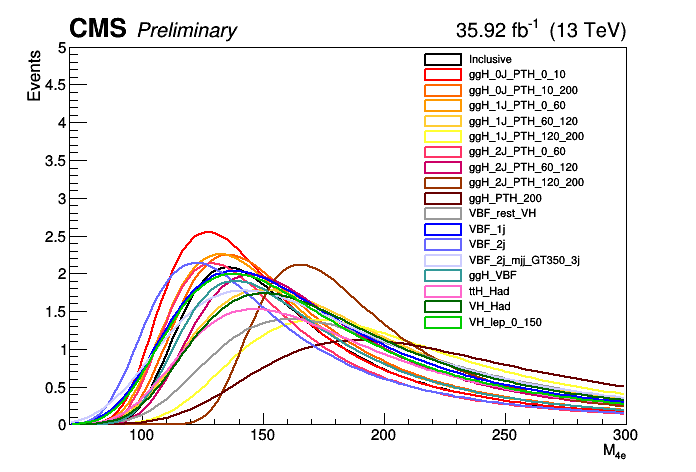
\includegraphics{Figures/RedBkg/allFits_data2016_4e.png}}}
%    \subfigure [] {\resizebox{7.75cm}{!}{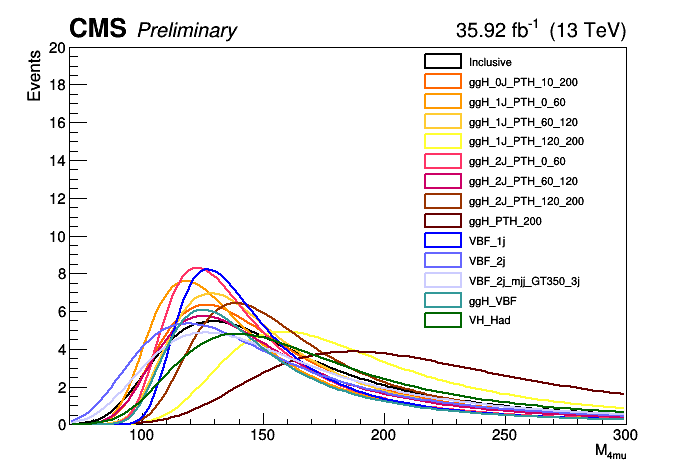
\includegraphics{Figures/RedBkg/allFits_data2016_4mu.png}}}\\
%    \subfigure [] {\resizebox{7.75cm}{!}{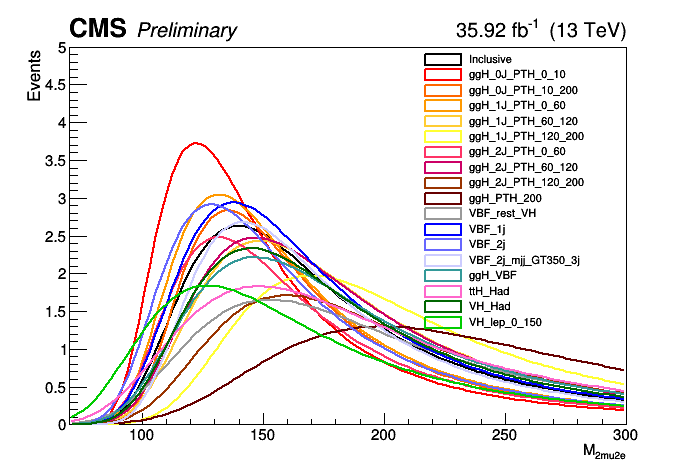
\includegraphics{Figures/RedBkg/allFits_data2016_2mu2e.png}}}
%    \subfigure [] {\resizebox{7.75cm}{!}{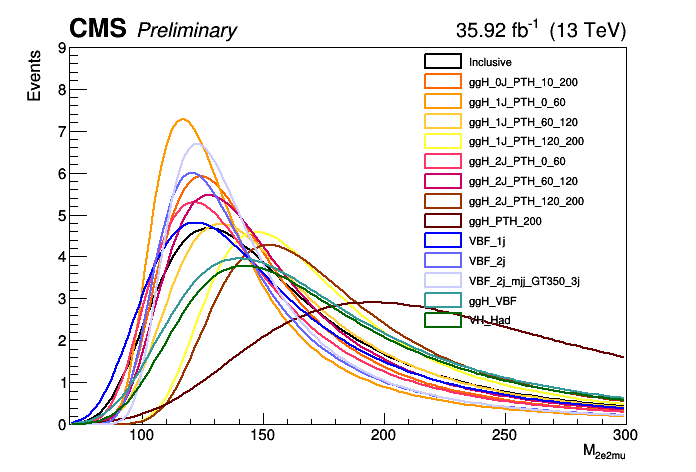
\includegraphics{Figures/RedBkg/allFits_data2016_2e2mu.png}}}
%\caption{Shapes of the $m_{4\ell}$ distribution for the reducible background in all the considered categories in the $4e$ (a), $4\mu$ (b), $2\mu2e$ (c) and $2e2\mu$ (d) final states using the SS method in the 2016 dataset.}
%\label{fig:shapes}
%\end{center}
%\end{figure}
%
On one hand, the results from the two methods are found to be more or less identical in the $4\mu$ and $2e2\mu$ final states; 
on the other hand, there is some difference in the $4e$ and $2\mu2e$ distributions but mainly due to a difference in the yields (Figure~\ref{fig:inclusiveComparison}). 
Taking into account the merged $2e2\mu$ and $2\mu2e$ final state, a fit to Landau function is still performed to obtain the $m_{4\ell}$ shape:
in fact, since the muon final state has a larger contribution, the addition of the $2\mu2e$ component does not distort the single Landau shape.

Looking at the comparison between the $m_{4\ell}$ distribution for the Z+X background obtained from the SS and OS methods in each category separately for all the final states,
shape differences between the two methods are found to be not significant. 
%Moreover, it is checked if the shape obtained from the SS method can reasonably describe the Z+X distribution given by the OS method considering each category individually: as an example, results for one category in all the considered final states are shown in Figure~\ref{fig:singleCatComparison}.

\begin{figure}[h]
\begin{center}
    \subfigure [] {\resizebox{7.75cm}{!}{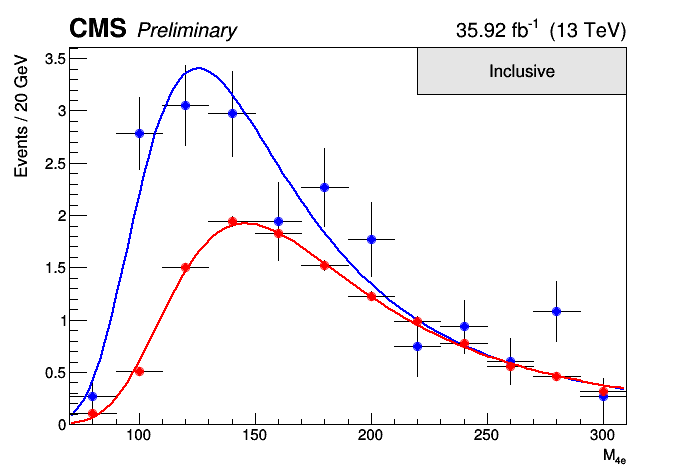
\includegraphics{Figures/RedBkg/fit_Inclusive_4e.png}}}
    \subfigure [] {\resizebox{7.75cm}{!}{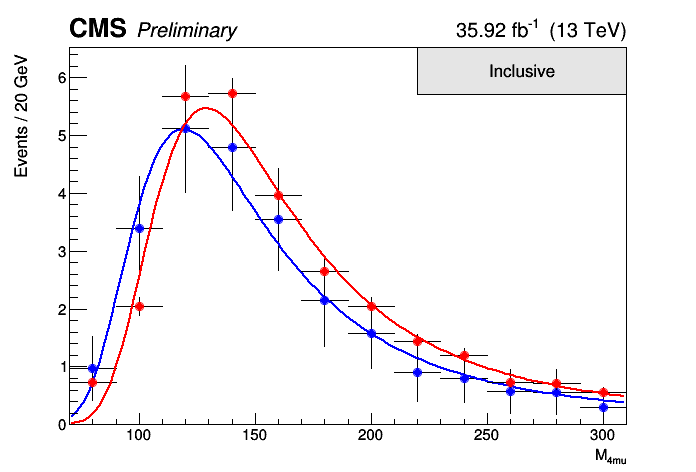
\includegraphics{Figures/RedBkg/fit_Inclusive_4mu.png}}}\\
    \subfigure [] {\resizebox{7.75cm}{!}{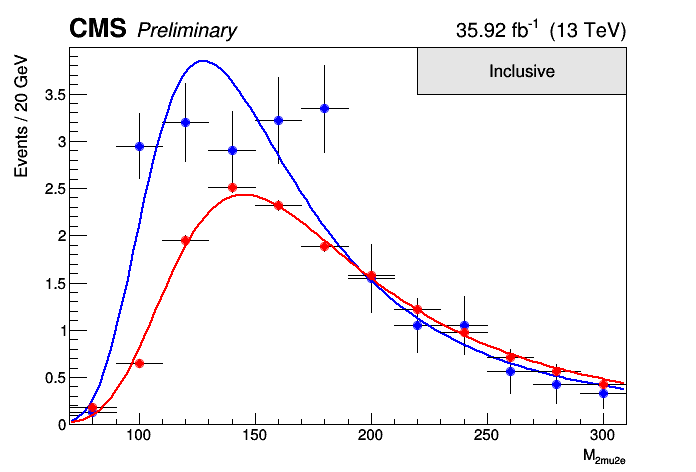
\includegraphics{Figures/RedBkg/fit_Inclusive_2mu2e.png}}}
    \subfigure [] {\resizebox{7.75cm}{!}{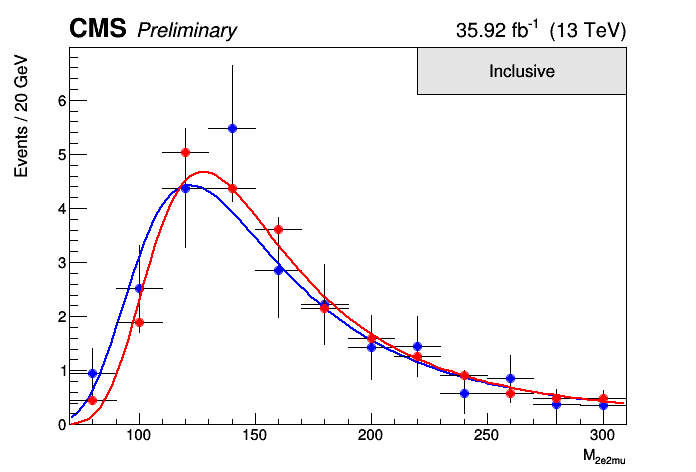
\includegraphics{Figures/RedBkg/fit_Inclusive_2e2mu.png}}}
\caption{Comparison between the $m_{4\ell}$ distribution for the Z+X reducible background obtained from the SS and OS methods (2016 dataset) in the inclusive category for each considered final state: $4e$ (a), $4\mu$ (b), $2\mu2e$ (c) and $2e2\mu$ (d).}
\label{fig:inclusiveComparison}
\end{center}
\end{figure}

%\begin{figure}[h]
%\begin{center}
%    \subfigure [] {\resizebox{5.1cm}{!}{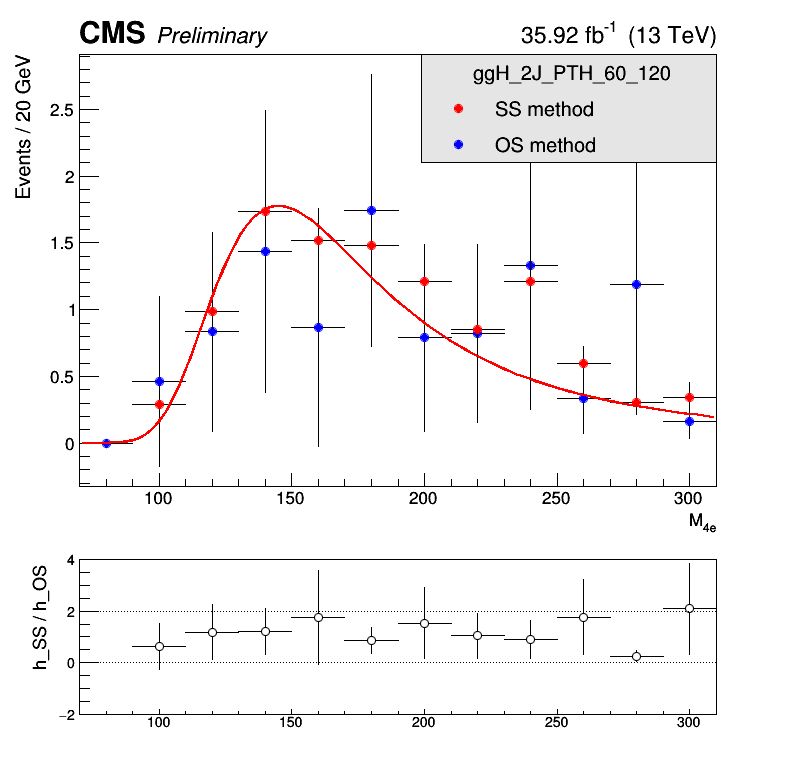
\includegraphics{Figures/RedBkg/fit_ggH_2J_PTH_60_120_4e.png}}}
%    \subfigure [] {\resizebox{5.1cm}{!}{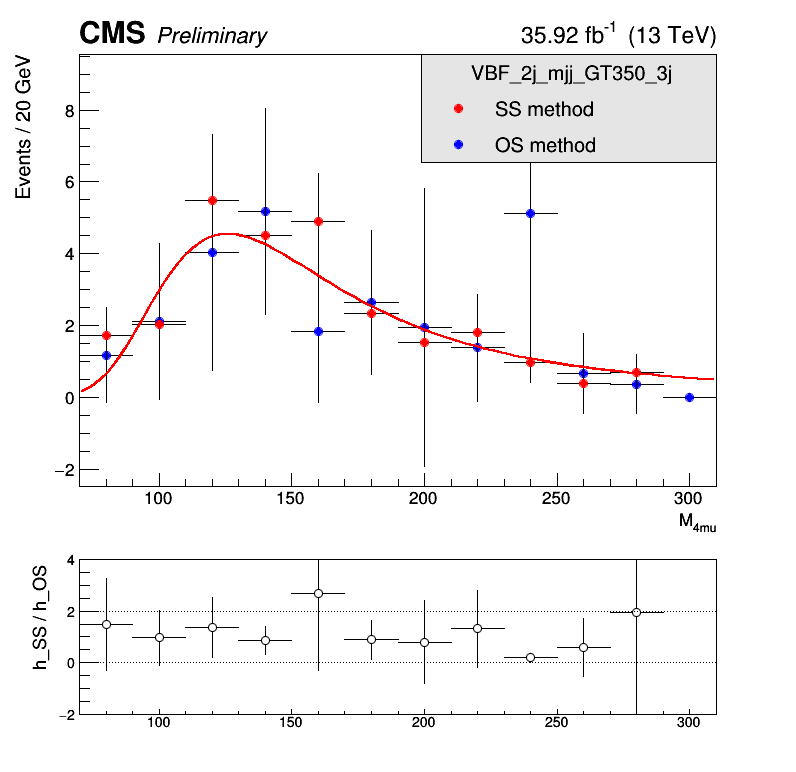
\includegraphics{Figures/RedBkg/fit_VBF_2j_mjj_GT350_3j_4mu.png}}}
%    \subfigure [] {\resizebox{5.1cm}{!}{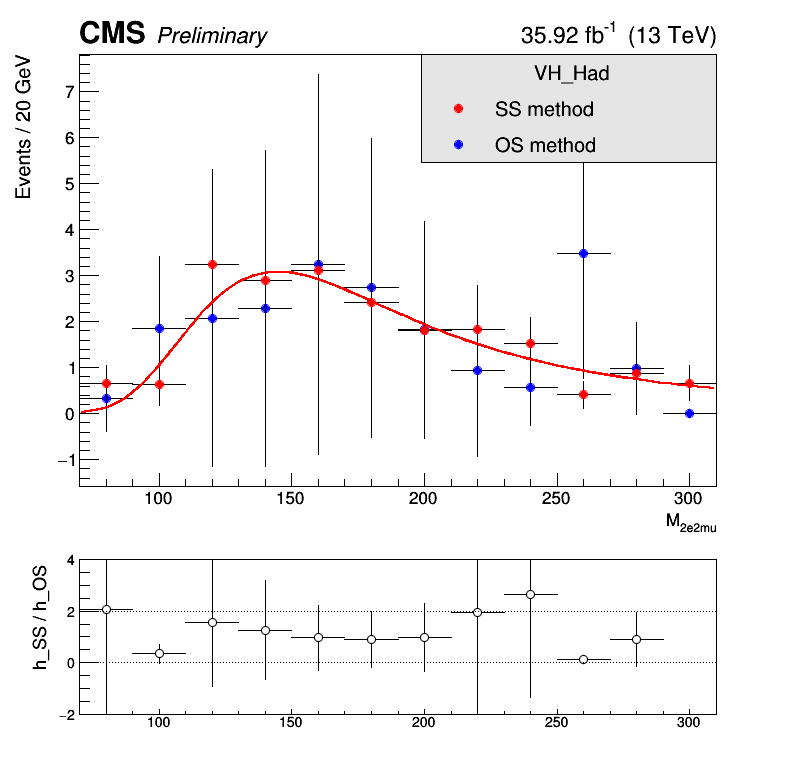
\includegraphics{Figures/RedBkg/fit_VH_Had_2e2mu.png}}}
%\caption{Comparison between the $m_{4\ell}$ distribution for the Z+X background obtained from the SS and OS methods (2016 dataset) fitted by the SS shape for the ggH$\_$2j$\_60\_120$ category in the $4e$ final state (a), for the VBF$\_$2j$\_$mjj$\_$GT350$\_$3j category in the $4\mu$ final state (b) and for the VH$\_$Had category in the $2e2\mu$ final state (c).}
%\label{fig:singleCatComparison}
%\end{center}
%\end{figure}


